\chapter{LITERATURE REVIEW}
\label{ch:literature}

% This is Chapter 2 - Literature Review
% Review relevant literature and related work in your field

\section{Introduction}

The growing demand for affordable analytics tools across all levels of football has attracted significant interest in research over the last few years. This effort is spearheaded by the YOLO (You Only Look Once) architecture for object detection, which has developed into a dominant architecture for real-time video object detection. This chapter reviews the current literature that provides the foundations for this thesis.

The review is organized as follows. Section 2.2 establishes the theoretical background by following the development of object detection from handcrafted feature description to the modern YOLO architecture. Section 2.3 surveys the related work, detailing the evolution of the YOLO architecture, its current implementation in football video object detection, prior studies on the benchmarks of models in hardware-constrained environments, and an overview of the dataset. Section 2.4 identifies the positioning of this study within the current literature, and Section 2.5 presents a summary of the major themes established in this review.


\section{Theoretical Background}

\subsection{From Traditional Methods to Deep Learning Detection}
Initial methods of detecting objects from video footage utilized handcrafted feature descriptors and classic machine learning classifiers. Dalal and Triggs (2005)\cite{RN03} introduced the Histogram of Oriented Gradients (HOG), which combined with Support Vector Machines (SVM) became the standard pipeline for such tasks. While computationally modest, these pipelines struggled with inconsistencies that come with video footage such as illumination variabilities, partial object occlusions and pose variations. These limitations would be exaggerated further in our application on football broadcast footage, due to the persistent occlusion of the ball or players by other players, pitch elements or the background. 

\begin{figure}[h]
    \centering
    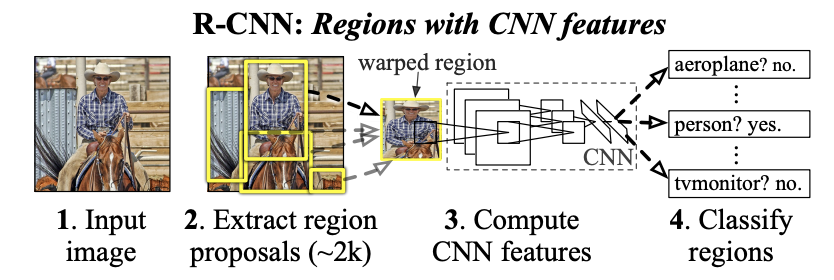
\includegraphics[width=1\textwidth]{figures/R-CNN.png}
    \caption{System overview of early R-CNN object detection (Girshick et al., 2014\cite{RN04}}
    \label{fig:R-CNN system}
\end{figure}

Convolutional Neural Networks (CNNs) however demonstrated that learning features from labelled data vastly outperforms handcrafted feature descriptions, as first showcased by Alex Krizhevsky (2012) \cite{RN05}, and subsequent architectures such as VGGNet and ResNet. In the same object detection domain, the Region-based CNN (R-CNN) architecture, developed by Girschick et al. (2014)\cite{RN04}, and refined in later versions into Fast R-CNN and Faster R-CNN, achieved what was for the time state-of-the-art accuracy by combining selective search regions with CNN classifiers. It proved computationally excessive for real-time detection however, with the two-stage pipeline requiring approximately 13 seconds per image on a GPU and 53 seconds per image on a CPU (Girschick et al., 2014)\cite{RN04}.

\subsection{Single-Stage detection: The YOLO paradigm}
\begin{figure}[h]
    \centering
    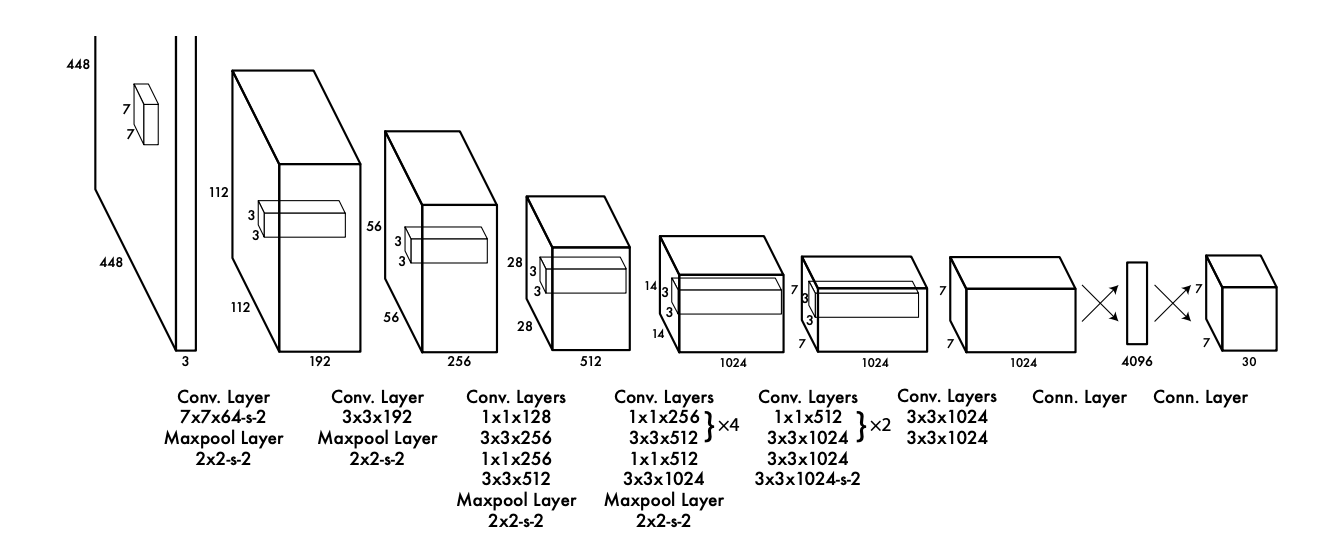
\includegraphics[width=1\textwidth]{figures/YOLO architecture.png}
    \caption{Architecture of the first YOLO model (Redmon et al., 2016)\cite{RN06}}
    \label{fig:YOLO architecture}
\end{figure}
The shift from two-stage detection to a single-stage approach was first introduced by Redmon et al. (2016)\cite{RN06} in the You Only Look Once (YOLO) publication. By tackling detection as a single regression problem, the You Only Look Once paradigm processes an entire frame in one forward pass, predicting box boundaries and class probabilities simultaneously. This removed the very costly step of region proposal completely, enabling the original YOLO detector to perform at 45 frames per second on a Titan X GPU. This was a dramatic speed improvement over R-CNN, though at a cost of lower accuracy on small objects.

Three concepts that make the foundations of the architecture evaluated in this thesis were introduced by the YOLO paradigm. 
\begin{enumerate}
\item The grid based prediction structure makes sure that spatial localization and classification are handled together, removing the computational drawback of a distinct proposal stage seen in earlier approaches.
\item Anchor boxes introduced in later models (Redmon and Farhadi, 2017)\cite{RN07}, supply prior bounding box shapes derived through k-means clustering. This means the model only needs to predict offsets rather than finding absolute coordinates. 
\item Multi-scale detection, introduced in YOLOv3 (Redmon and Farhadi, 2018)\cite{RN08}, managed to significantly improve small object detection, a previous limitation of the YOLO architecture, through the use of feature maps at three different resolutions.
\end{enumerate}

\subsection{Target Performance Metrics}
Object detection models are evaluated using two primary standard metrics. Mean Average Precision (mAP) provides a summary of detection quality across all classes and Intersection over Union (IoU) thresholds. The mAP@0.5 metric is computed at an IoU threshold of 0.5. It constituted a simple indication of whether the detector’s produced bounding boxes are substantially overlapping with known ground truth. The mAP@0.5:0.95 metric is a stricter version of mAP@0.5, averaging precision across IoU thresholds from 0.5 to 0.95. It penalizes imprecise localization and provides a more demanding picture of detection accuracy.

Inference speed is defined as latency per image in milliseconds or its reciprocal, frames per second (FPS). For deployment on consumer hardware, both CPU and GPU latency figures are relevant, as the compute capabilities of consumer devices span a wide spectrum from integrated graphics to discrete GPUs. 

The trade-off between mAP and inference latency makes up the central analytical domain of this study, and these metric definitions therefore form the evaluative vocabulary upon which the comparative analysis is built.

\section{Related Work}

\subsection{The Evolution of the YOLO Architecture}
Following the original YOLO detector, successive versions introduced targeted improvements that progressively narrowed the accuracy gap between single-stage and two-stage approaches, especially when targeting small objects. The work that gave us YOLOv4 (Bochkovskiy et al., \cite{RN09}) consolidated a large body of practices, including the CSPDarknet53 backbone, a PANet neck for improved feature pyramid fusion, Mosaic data augmentation, and the CioU (Complete Intersection over Union) loss function, into a unified architecture that set a new state-of-the-art among real-time object detectors on the MS COCO benchmark.

YOLOv8, released by Ultralytics in January 2023\cite{RN10}, represents the architectural base upon which this thesis is built. It introduced several significant refinements over preceding models. The backbone replaces the C3 (Cross Stage Partial with three convolutions) module with a a redesigned Cross Stage Partial (C2f) module that improves feature reuse and gradient propagation through more efficient cross-stage connections and lightweight bottleneck layers. This design improves gradient flow during training and reduces parameter count relative to the previous CSP blocks. The neck retains a PANet-based feature pyramid and retains the Spatial Pyramid Pooling Fast (SPPF) module introduced in latter models of YOLOv5 to efficiently capture multi-scale context. The detection head represents the most consequential architectural change: YOLOv8 adopts an anchor-free, decoupled head that separately predicts bounding box regression and object classification. By eliminating predefined anchor boxes, the model generalizes more readily to custom datasets where object aspect ratios differ from those of the general-purpose COCO training set, a property of particular value when fine-tuning on a domain-specific dataset.

YOLOv8 is offered in five variants, each in a different scale: nano, small, medium, large and extra large. The models are scaled by adjusting the width and depth of the backbone and neck. The scaling is set such as each following step increases in magnitude from the previous in both parameter count and mAP scores. This behaviour makes this architecture suitable for comparative studies as the topologu is held constant while only the model capacity differs.


\subsection{YOLOv8 Variant Comparisons}
Previous studies have systematically compared YOLOv8 variants across different hardware configurations and application domains, providing an empirical context for the present thesis. Alqahtani et al. (2024)\cite{RN11} conducted a comprehensive benchmarking study of YOLOv8 variants (Nano, Small, and Medium) alongside EfficientDet Lite and SSD MobileNet models, deployed on Raspberry Pi 3, 4, and 5 devices with and without TPU (Tensor Processing Unit) accelerators, as well as on a Jetson Orin Nano. Their findings confirmed that lower-capacity models such as YOLOv8n deliver substantially lower inference latency and energy consumption, while higher-capacity models such as YOLOv8m provide superior mAP at the cost of increased computational overhead. Most importantly, they also identified that the model rank in regard to inference speed is largely dependant on the hardware environment, with different processing units resulting in different efficiency profiles.

Concretely on our football domain, a variant comparison was conducted by Tanapatpiboon et al. (2025)\cite{RN12} through football player detection and heatmap generation. The authors evaluated YOLOv5m6, YOLOv5l-tph, and related variants on broadcast footage and showed that YOLO object detection can succesfully be utilized in this application. However, they only focused on tracking team positions and ignored important information like the ball position and the distinction of the goalkeeper.

Ahmad Yousef et al. (2025)\cite{RN13} conducted a rigorous comparison of the YOLOv8x (extra-large) and YOLOv12x models on the task of football analytics. Their results also confirmed the consistent pattern of larger models with more parameters achieving higher accuracy scores while requiring more computational capacity. 

\begin{figure}[h]
    \centering
    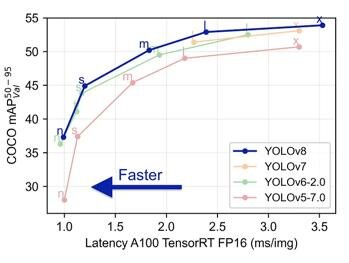
\includegraphics[width=0.8\textwidth]{figures/YOLO_model_comp.png}
    \caption{A comparison between YOLOv8 and other YOLO models (Ultralytics, 2023)\cite{RN10}}
    \label{fig:YOLO_model_comp}
\end{figure}
The aforementioned pattern was also confirmed by Markappa et al. (2024)\cite{RN14}, who conducted a comparison on the different architectures of YOLO models, namely YOLOv3, YOLOv5, YOLOv8, and YOLOv9. This comparison was made on the SoccerNet dataset, and their findings showed interestingly that the YOLOv8 models were able to achieve higher accuracy than the successor, YOLOv9, however this also came at the cost of higher inference latency.

\subsection{YOLO Based Detection in Football Video Footage}
The YOLO architecture has been proven to be very impressive in the football domain. The performance evaluation conducted by Tshiani (2025)\cite{RN15} provides class-level mAP benchmarks from a YOLOv8s-based pipeline trained and evaluated on a custom dataset combining Bundesliga, NCAA Division I, and UPSL broadcast footage. Tshiani reported mAP@0.5 values of 0.993 for player detection, 0.946 for referees, 0.931 for goalkeepers, and only 0.616 for the ball class, highlighting that across all evaluated classes, ball detection remains the most challenging task, primarily due to its small spatial footprint and frequent occlusion. 

The same challenge was found in the study made by Ahmad Yousef et al. (2025)\cite{RN13}. In their comparison between the different YOLO models, ball detection proved to be the most difficult task, with distinctly lower accuracy scores across the different models. However, a solution was found through the addition of a Kallman Filter to the pipeline, which produced significant improvement in the F1-scores for the ball class.

Another study depicting the same difficulties was made from Hartono et al. (2025)\cite{RN16}. They used an integrated YOLOv5 pipeline for player tracing, team assignment and speed estimation. As seen in the aforementioned studies, player detection was impressive (this study showed player detection accuracy of 94.8\%), however ball detection was very difficult with a precision-recall score of 0.478

\subsection{YOLOv8 Variant Scaling}
A recurring theme in the YOLO benchmarking literature is the hardware dependence of inference performance, which motivates the consumer-hardware framing of the present thesis. According to official Ultralytics (2023)\cite{RN10} documentation, the YOLOv8n model offers a latency of under 1 ms on a A100 TensorRT GPU. However, these figures are not representative of the inference conditions experienced by a university student, a football academy analyst, or an amateur club coach operating on commodity hardware. Consumer hardware, defined for the purposes of this thesis as mid-range laptops and desktop systems equipped with budget discrete GPUs and integrated graphics, presents a qualitatively different deployment context.

This is where the different scales of the YOLOv8 family come into use. By gradually increasing the parameters and FLOPs (Floating Point Operations), we can aim to find the most effective model for our hardware and usage.

\begin{table}[H]
    \centering
    \label{tab:yolov8_variants}
    \begin{tabular}{lcccccc}
        \hline
        \textbf{Model} & \textbf{Size} & \textbf{mAP\textsuperscript{val}} & \textbf{Speed CPU} & \textbf{Speed A100} & \textbf{Params} & \textbf{FLOPs} \\
                       & \textbf{(px)} & \textbf{50-95}                    & \textbf{ONNX (ms)} & \textbf{TensorRT (ms)} & \textbf{(M)} & \textbf{(B)} \\
        \hline
        YOLOv8n & 640 & 37.3 & 80.4  & 0.99 & 3.2  & 8.7   \\
        YOLOv8s & 640 & 44.9 & 128.4 & 1.20 & 11.2 & 28.6  \\
        YOLOv8m & 640 & 50.2 & 234.7 & 1.83 & 25.9 & 78.9  \\
        YOLOv8l & 640 & 52.9 & 375.2 & 2.39 & 43.7 & 165.2 \\
        YOLOv8x & 640 & 53.9 & 479.1 & 3.53 & 68.2 & 257.8 \\
        \hline
    \end{tabular}
    \caption{YOLOv8 model variants and their performance metrics (Ultralytics, 2023)\cite{RN10}.}
\end{table}

Shuvo et al. (2022)\cite{RN17} identify several established strategies for deploying deep learning models on resource-constrained devices, including pruning, quantization, knowledge distillation, and compact architecture design. Of these, selecting among pre-scaled model variants (the approach taken in this thesis) requires no modification to the model or training pipeline, making it the most practically accessible option for users without specialized engineering expertise.


\subsection{The Bundesliga Data Shootout dataset}
The Bundesliga Data Shootout dataset, published on Roboflow Universe by Delfos (2022)\cite{RN18} and derived from the DFL Kaggle competition, provides YOLO-format annotations for the player, referee, goalkeeper, and ball classes. Because of its quality and relevance, it is the most used in modern computer vision studies inside the football context, making it the most contextually relevant publicly available benchmark for this work.

\section{Positioning of the Present Study - Summary}

The review conducted in this chapter traces the development of object detection approaches from rudimentary handcrafted methods like HOG combined with SVMs, progressing into the R-CNN two-stage process, finally maturing into the YOLO paradigm which delivers strong accuracy while achieving real-time video processing. Within that paradigm the current YOLOv8 proves to be the best, achieving impressive accuracy scores and offering different scale models in order to adapt to different tasks and environments that practitoners have.

Its application to football analytics is recent and well established. Markappa et al. (2024)\cite{RN14} confirm that YOLOv8 consistently outperforms earlier versions on football-specific data, while Tshiani (2025)\cite{RN15}  and Ahmad Yousef et al. (2025)\cite{RN13} provide the closest empirical comparators to the present work, establishing that player detection approaches saturation across model sizes while ball detection remains the persistent challenge of the domain.

The review also reveals that existing comparisons of these YOLOv8 variants are not fully adapted to the task we are aiming to achieve, which is to implement the YOLOv8 models into consumer grade hardware. From our investigation, these comparisons are either made in datasets unrelated to football footage, which means they miss the specific challenges such a task poses, or they are conducted on very expensive hardware configurations, meaning that the models might not be viable to the target demographic. 

The present thesis addresses these questions through a controlled evaluation of YOLOv8n, YOLOv8s, and YOLOv8m on the Bundesliga Data Shootout dataset, conducted specifically on consumer-grade hardware across three different price points, with the aim of providing practical model selection guidance for users operating under realistic resource constraints
